\section{Descrizione generale}

\subsection{Obiettivi del prodotto}
Il nome del servizio è \textit{Etherless} ed sviluppato con una architettura decentralizzata\glo.\\ \textit{Etherless} permette agli sviluppatori di caricare funzioni JavaScript\glo sul cloud\glo per poi renderle disponibili ad utenti terzi (utilizzatori). Il servizio si presenta come un CaaS\glo (Computation\glo-as-a-Service) in cui l’utilizzatore paga per la singola esecuzione di una funzione in modo automatico mediante l’utilizzo della rete Ethereum\glo e degli smart contract\glo. Una parte del compenso viene accreditata allo sviluppatore e una parte viene trattenuta da \textit{Etherless}.

\subsection{Funzioni del prodotto}
L'obbiettivo finale è quello di avere un ambiente in cui lo sviluppatore \textit{Bob}, dopo aver sviluppato una funzionalità che potrebbe essere di interesse per altri sviluppatori (es. \textit{Alice}), carica il suo codice JavaScript su \textit{Etherless} mediante la sua utenza e imposta un costo di esecuzione per quella funzione. \textit{Alice}, abile programmatrice, siccome ha bisogno di tale funzionalità, decide che conviene pagare la quota di esecuzione piuttosto che riscrivere la stessa procedura; attraverso la sua utenza \textit{Etherless}, \textit{Alice} è quindi capace di usufruire della funzione in cloud e sostenere il costo di esecuzione che viene tassato ad ogni singola chiamata di funzione.
\\\\
Non c'è differenziazione fisica tra gli utenti del servizio ed entrambi sono rappresentati da un account Ethereum\glo, composto quindi da un indirizzo e da una chiave privata. Possiamo fare una distinzione logica tra l'utente \textbf{sviluppatore}, che decide di rendere pubblica una o più funzioni, e l'utente \textbf{utlizzatore} che invece decide di utilizzare funzioni altrui. La differenziazione avviene solamente nell'instante in cui intraprende una azione. 
\\In generale l'utente può:
\begin{itemize}
	\item registrarsi al servizio richiedendo un nuovo account;
	\item accedere alla sua utente inserendo le sue credenziali di accesso;
\end{itemize}
\\In particolare
\begin{itemize}
	\item l'utente sviluppatore può
	\begin{itemize}
		\item elencare le funzioni da lui rese pubbliche;
		\item creare una nuova funzione e specificarne nome e costo di esecuzione;
		\item caricare il codice relativo ad una sua funzione;
		\item eliminare una funzione da lui pubblicata;
		\item visualizzare il log delle chiamate alle sue funzioni
	\end{itemize}
	\item l'utente utilizzatore può
	\begin{itemize}
		\item elencare tutte le funzioni disponibili;
		\item eseguire una funzione tra quelle disponibili;
		\item eseguire il logout della sua utenza;
	\end{itemize}
\end{itemize}


\subsection{Caratteristiche}
\subsubsection{Caratterische utenti}
\subsubsection{Identificazione}
Gli utenti \textit{Etherless} sono identificati univocamente attraverso un account Ethereum\glo. Questo significa che un account utente non è identificato e caraterrizzato da parametri comuni (nome, cognome, email, password, etc.) ma da una combinazione di \textit{address} e \textit{private-key}\glo specifici delle reti blockchain.
\subsubsection{Autenticazione}
Per la persistenza della sessione dell'utente, verranno salvati nel file system del computer le credenziali di accesso in seguito alla registrazione o all'accesso dell'utente su una istanza \textit{etherless-cli}
\begin{itemize}
	\item \textbf{Accesso}: nel caso l'utente voglia accedere alla sua utenza \textit{Etherless}, gli verrà chiesto di inserire le sue credenziali
	\item \textbf{Registrazione}: nel caso della registrazione di una nuova utenza, verrà inoltrata la richiesta alla rete Ethereum\glo che genererà un combinazione di credenziali univoca;
\end{itemize}
\subsubsection{Crediti}
Ogni utente ha associato al suo account un certo numero crediti (ether\glo). Non è stato richiesto di prevedere una modalità di ricarica dei crediti. Ogni account, alla sua creazione avrà un a disposizione un certo numero di ether\glo.

\subsection{Caratteristiche tecniche}
La piattaforma deve essere conforme a quanto segue:
\begin{itemize}
	\item gli utenti avranno la possibilità elencare le funzioni disponibili,  caricarne di nuove, aggiornarle, eseguirle oppure eliminare attraverso \textit{etherless-cli};
	\item utilizzo della rete \textit{Ethereum}\glo per la comunicazione tra i vari componenti di \textit{Etherless}, per la definizione della logica di interazione tra le varie parti (smart contract\glo) e per lo storage\glo di dati;
	\item per la realizzazione dell backend deve essere prevista una infrastruttura Serverless\glo;
	\item Utilizzo del servizio AWS Lambda per lo storage\glo ed esecuzione in cloud\glo delle funzioni caricate;
	\item La comunicazione tra i vari componenti di \textit{Etherless} deve avvenire solamente attraverso eventi Ethereum\glo; TODOOOOOO INSERIREI LA LORO IMMAGINEEE

\end{itemize}
A questo proposito, per la realizzazione del servizio sono previste la realizzazione di tre applicativi software:
	\begin{itemize}
		\item \textbf{\textit{etherless-cli:}} interfaccia a linea di comando attraverso la quale gli utenti si interfacciano con il servizio ed eseguono le funzionalità disponibili;
		\item \textbf{\textit{etherless-smart:}} applicativo che si occupa della definizione e del deploy\glo dello smart contract sulla rete Ethereum;
		\item \textbf{\textit{etherless-server:}} applicativo server che ascolta e soddisfa le richieste di esecuzione delle funzioni caricate interfacciandosi con il servizio AWS Lambda mediante l'apposito SDK;
	\end{itemize}
\subsubsection{Trasferimento del denaro}
La granularità di accredito deve essere per singola chiamata di funzione. Inoltre, sono state individuate due modalità di trasferimento del denaro dall'utilizzato allo sviluppatore della funzione richiamata:
\begin{itemize}
	\item trasferimento diretto dei fondi quando il contratto riceve la richiesta di esecuzione
	\item mediante escrow: i soldi vengono prelevati dall'utilizzatore alla ricezione della richiesta di esecuzione e accreditati allo sviluppatore solamente quando l'output della funzione richiesta raggiunge l'utilizzatore.
\end{itemize}
Il committente ha specificato che la prima versione è accettata.

\subsubsection{Archiviazione dei dati}
Per lo storage\glo dei dati non è previsto l'utilizzo di database. Emerge dall'analisi fatta sulle specifiche richieste che non è necessario il salvataggio di dati di lungo formato (quali immagini o descrizioni). Informazioni come nomi di funzioni, ownership\glo e costi di esecuzioni vengono salvati direttamente sulla rete Ethereum\glo attraverso lo smart contract\glo; 
\\\\
Nel caso in cui durante la fase di sviluppo del progetto sorga la necessità di salvare quantitativi più grandi di dati, verra utilizzato un database relazionale o non-relazionale disponibile sotto Amazon Web Services;
\subsubsection{Accesso alle risorse}
\begin{itemize}
	\item L'utente in generale ha accesso a tutte le funzioni pubblicate: vederne il nome, i parametri richiesti, e richiederne l'esecuzione;
	\item Lo sviluppatore, sulle funzioni di sua proprietà può: vederne il nome e parametri associati, caricare e modificare il codice, eliminare una funzione e crearne di nuove;
	\item Alle risorse disponibili su AWS hanno accesso solo \textit{etherless-cli} e \textit{etherless-server};
\end{itemize}
\subsubsection{Tecnologie}
Tecnologie da utilizzare
\begin{itemize}
	\item \textbf{AWS (Amazon Web Services)}: piattaforma che si occupa di fornire servizi di cloud computing\glo;
	\item \textbf{AWS - Lambda}: servizio che consente di eseguire codice nel cloud;
	\item \textbf{Ethereum}: una rete globale per il trasferimento di criptovalute\glo e per la realizzazione di applicativi decentralizzati
	\item \textbf{Solidity}: linguaggio OOP\glo per la definizione di smart contract\glo;
	\item \textbf{Truffle}: framework per lo sviluppo di smart contract su rete Ethereum\glo;
	\item \textbf{Web3}: API\glo JavaScript per l'interazione con un noto Ethereum\glo locale o remote;
	\item \textbf{Ropsten}: Rete Ethereum\glo pubblica usato per il testing di applicativi Ethereum\glo prima del porting\glo in produzione sulla \textit{MainNet};
	\item \textbf{MainNet}: Rete Ethereum\glo principale;
	\item \textbf{Ganache}: Ambiente di sviluppo Ethereum\glo utilizzato per la simulazione locale si una rete Ethereum\glo e per l'analisi delle transazioni e log;
	\item \textbf{TypeScript 3.6}: versione standardizzata da Microsoft del linguaggio JavaScript;
	\item \textbf{Node.js}: ambiente di runtime open-source per JavaScript;
	\item \textbf{The Serverless Framework}: framework per la costruzione e deploy\glo (anche su AWS) di ambienti serverles\glo;
	\item \textbf{Smart Contract}: protocollo informatico che facilita, verifica, fa rispettare ed esegue un contratto (insieme di regole);
	\item \textbf{ESLint}: strumento di analisi del codice utilizzato per identificare pattern\glo problematici nel codice JavaScript;
\end{itemize}
\subsection{Ambienti}
Il cliente ha richiesto la possibilità di eseguire il programma nelle seguenti modalità:
\begin{itemize}
	\item \textbf{locale:} simulando una rete Ethereum\glo sulla propria macchina;
	\item \textbf{test:} simulando una rete Ethereum\glo su un ambiente di test condiviso tra gli sviluppatori del progetto;
	\item \textbf{staging:} utlizzando un rete Ethreum\glo di test pubblica come Ropsten\glo;
	\item \textbf{production:} utilizzando la rete Ethereum\glo ufficiale MainNet\glo;
\end{itemize}
A tale scopo deve essere prevista la configurazione dei vari ambienti su \textit{etherless-smart}, \textit{etherless-cli} e \textit{etherless-server}.
\subsection{Architetture del progetto}
Come già anticipato, le componenti necessarie per la realizzazione di \textit{Etherless} sono \textit{etherless-cli, etherless-smart} e \textit{etherless-server}. L'architettura del servizio sarà quella di una app decentralizzata\glo (DApp\glo). Le DApp\glo girano su una rete di computer P2P piuttosto che su un singolo computer, sfruttando la tecnologia blockchain\glo.\\
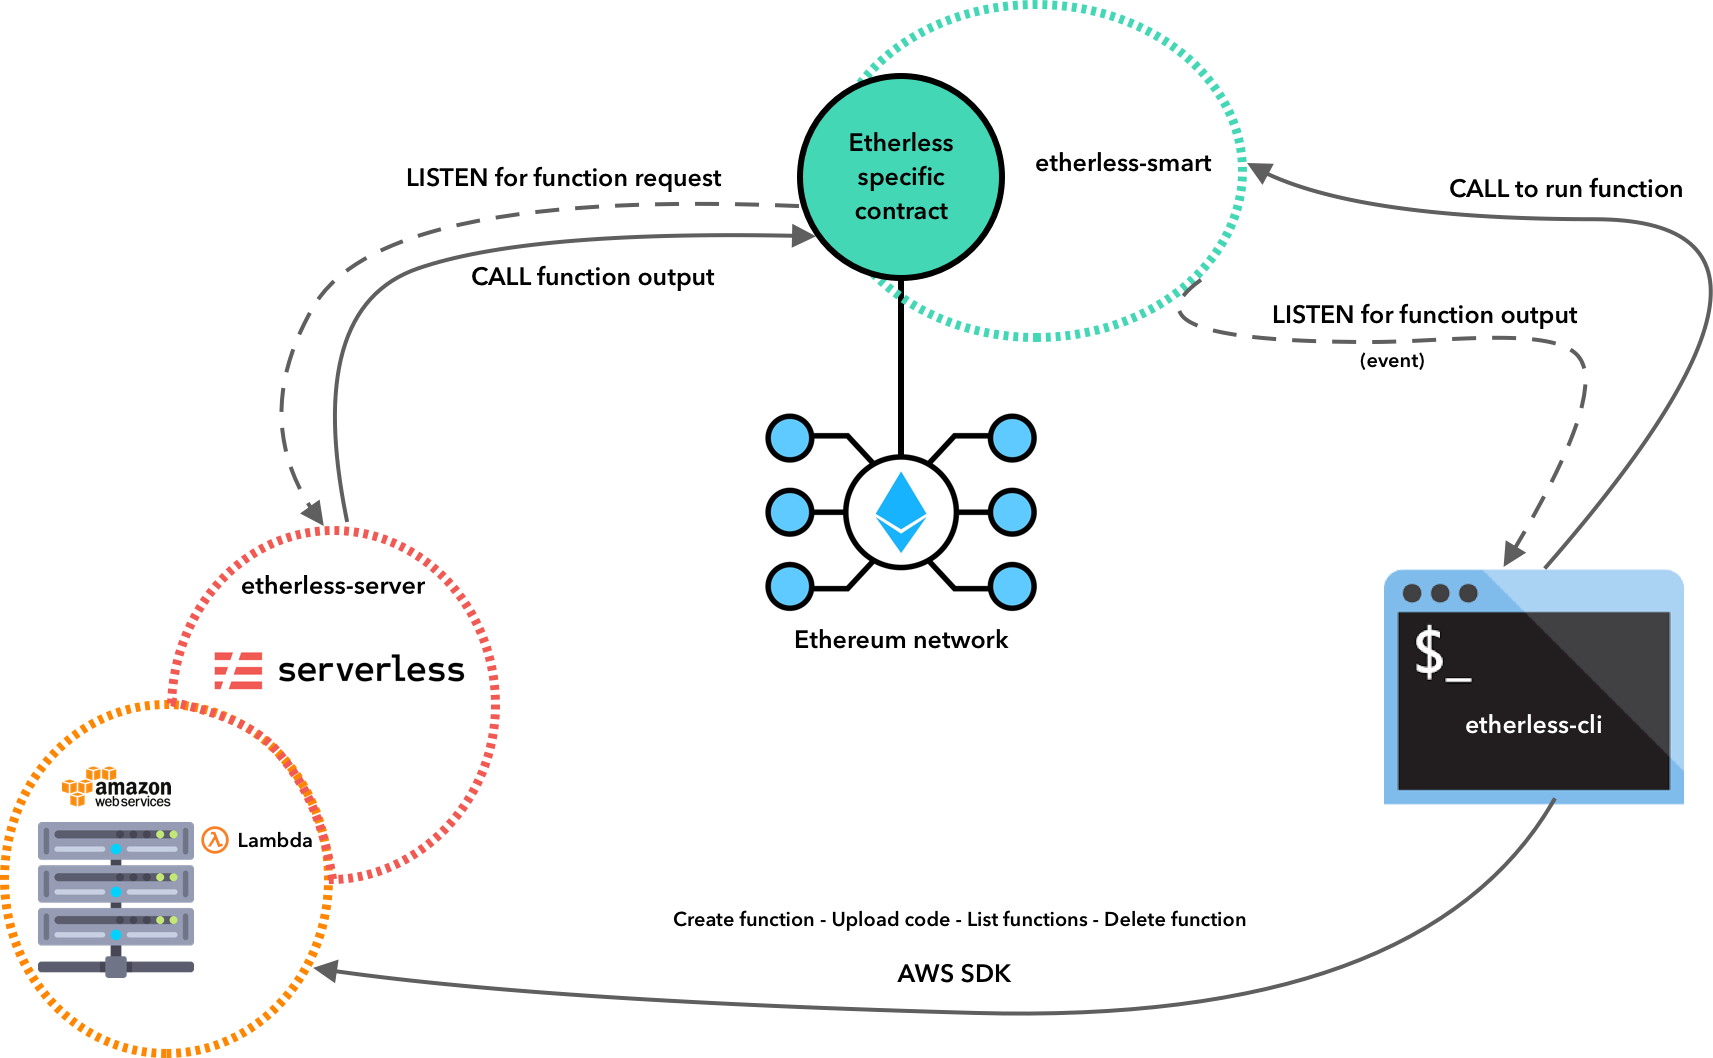
\includegraphics[width=\textwidth]{res/img/archi}
\subsubsection{Etherum\glo network}
Il servizio baserà il suo funzionamento su uno {smart contract}\glo che si occuperà di regolare indirettamente le interazioni tra sviluppatori, e in modo diretto gesiticse l'esecuzione delle funzioni e l'interazione dell'utente con il servizio. Inoltre, lo smart contract viene usato anche come storage per i dati dell'applicazione. Una volta definite le regole del contratto, questo viene reso pubblico mediante la sua compilazione e deploy\glo sul network\glo. Questa operazione ci fa ottenere l'indirizzo (address) del contratto nella rete e l'ABI\gli del contratto stesso. Questi dati saranno utili a \textit{etherless-cli} e \textit{etherless-server} per potersi interfacciare il contratto stesso.
\subsubsection{Front-end}
L'interazione dell'utente con con il servizio avviene attraverso una interfaccia a linea di comando (CLI\glo) e tale applicativo prende il nome di \textit{etherless-cli}. L'utilizzo è di tipo richiesta e risposta: l'utente avvia il processo digitando un comando specifico, l'applicativo ricava l'output corrispondente, lo mostra a video e poi interrompe la sua esecuzione. \\Per completare la richiesta dell'utente, il processo può richiamare funzioni del contratto oppure mettersi in ascolto di eventi sulla rete Ethereum\glo.
\\Nel caso in cui l'utente sia uno sviluppatore e viene richiesta la creazione di una nuova funzione, questo componente sarà in grado di usare l'sdk\glo di AWS per caricare la funzione su AWS Lambda\glo.
\subsubsection{Serverless}
Quando il contratto riceve una richiesta di esecuzione di una funzione remota, viene emesso un evento che specifica il nome della funzione e i paramateri con cui eseguire tale procedura. Questi tipi di eventi vengono ascoltati da \textit{etherless-server}. Una volta ricevuto viene utilizzato l'sdk\glo di AWS per ottenere il risultato dell'esecuzione della funzione stessa. Tale risultato viene emesso sulla rete dal contratto in modo che \textit{etherless-cli} possa leggerlo e mostrarlo all'utente richiedente.
\\\\
\textit{etherless-server} è processo che verrà messo in esecuzione continua in un ambiente serverless, utilizza il framework Serverless e impostando AWS come destinazione del deploy\glo.
\subsubsection{Schema di interazione}
Di seguito viene mostrato quale deve essere il flusso delle interazioni dei vari componenti.\\
	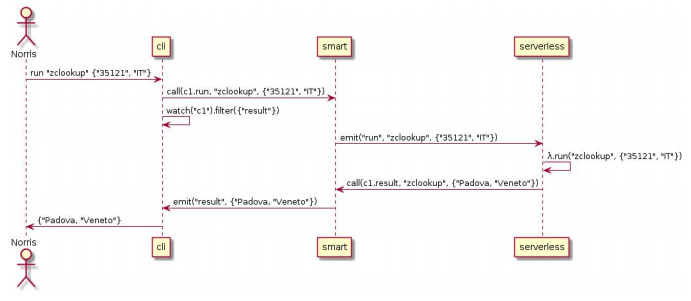
\includegraphics[width=\textwidth]{res/img/calls-flow}
\subsection{Vincoli del sistema}
\subsubsection{Per l'utente}
Per l'esecuzione è necessaria una connessine ad Internet, l'installazione di node.js, e il download\glo di \textit{etherless-cli}. Per accedere al servizio l'utente dovrà prima creare una utenza oppure accedere con una già esistente. Preferibilmente richieste conoscenze nell' utilizzo del terminale\glo.
\subsubsection{Per il servizio}
Per l'esecuzione serverless del servizio è richiesta una utenza AWS e la corretta configurazione di tale ambiente. Inoltre, è necessario poter accedere a un network Ethereum\glo al quale appoggiare il servizio.
	
	